\documentclass[10pt]{beamer}

\usetheme{Madrid}
\usecolortheme{whale}
\usepackage{appendixnumberbeamer}
\usepackage{booktabs}
\usepackage[scale=2]{ccicons}
\usepackage{pgfplots}
\usepgfplotslibrary{dateplot}
\pgfplotsset{compat=1.18}

\usepackage{graphicx}
\usepackage{fontawesome5}
\usepackage{tikz}
\usetikzlibrary{positioning,arrows,shapes,decorations.pathreplacing}



\title{Policy Conflicts and Strategies in the Policy-Making Process}
\subtitle{Introduction to Public Policy}
\author{Dr. David Adams}
\institute{POSC 315 – Week 13}
\date{\today}

\begin{document}

\begin{frame}
    \titlepage
    \begin{quote}
        \small "Understanding and managing conflict is key to successful policymaking."
    \end{quote}
\end{frame}

\begin{frame}{Learning Objectives}
    \begin{itemize}[<+->]
        \item Understand the \textbf{sources} of policy conflict
            \only<1>{\faIcon{bolt}}
        \item Explore \textbf{strategies} to manage or resolve policy conflicts
            \only<2>{\faIcon{bullseye}}
        \item Reflect on how conflict can serve as both a \textbf{challenge} and an \textbf{opportunity}
            \only<3>{\faIcon{lightbulb}}
        \item Develop a foundation for applying these concepts to \textbf{real-world policy issues}
            \only<4>{\faIcon{check}}
    \end{itemize}
\end{frame}

\begin{frame}{What is Policy Conflict?}
    \begin{block}{Definition}
        A situation where stakeholders have opposing interests, goals, or values.
    \end{block}
    
    \begin{columns}[T]
        \begin{column}{0.5\textwidth}
            \textbf{Key Elements:}
            \begin{itemize}
                \item \textbf{Competing Interests}
                \item \textbf{Value Clashes}
                \item \textbf{Limited Resources}
            \end{itemize}
        \end{column}
        \begin{column}{0.5\textwidth}
            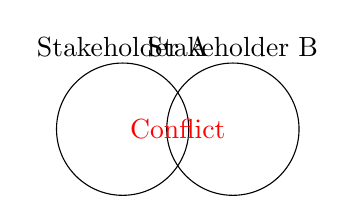
\begin{tikzpicture}[scale=0.7]
                \draw (0,0) circle (1.2);
                \draw (2,0) circle (1.2);
                \node at (0,1.5) {Stakeholder A};
                \node at (2,1.5) {Stakeholder B};
                \node[red] at (1,0) {Conflict};
            \end{tikzpicture}
        \end{column}
    \end{columns}
\end{frame}

\begin{frame}{Common Sources of Conflict}
    \begin{columns}[T]
        \begin{column}{0.5\textwidth}
            \begin{enumerate}
                \item \textbf{Differing Stakeholder Interests}
                \begin{itemize}
                    \item Business vs. Environmental Goals
                \end{itemize}
                
                \item \textbf{Ideological Differences}
                \begin{itemize}
                    \item Healthcare Debates
                \end{itemize}
            \end{enumerate}
        \end{column}
        \begin{column}{0.5\textwidth}
            \begin{enumerate}\setcounter{enumi}{2}
                \item \textbf{Resource Limitations}
                \begin{itemize}
                    \item Budget Competition
                \end{itemize}
                
                \item \textbf{Regulatory Constraints}
                \begin{itemize}
                    \item Jurisdictional Overlap
                \end{itemize}
            \end{enumerate}
        \end{column}
    \end{columns}
\end{frame}

\begin{frame}{Stakeholder Interest Conflicts}
    \begin{block}{Environmental Policy Example}
        \begin{itemize}
            \item Conflict: Economic development vs. conservation
            \item Stakeholders: Industry, environmental groups, communities
        \end{itemize}
    \end{block}
    
    \begin{block}{Social Policy Example}
        \begin{itemize}
            \item Conflict: Equity vs. efficiency in welfare programs
            \item Stakeholders: Taxpayers, beneficiaries, policymakers
        \end{itemize}
    \end{block}
\end{frame}

\begin{frame}{Ideological Clashes in Policy}
    \begin{block}{Examples}
        \begin{enumerate}
            \item \textbf{Healthcare Reform}
            \begin{itemize}
                \item Individual responsibility vs. collective welfare
            \end{itemize}
            
            \item \textbf{Tax Policies}
            \begin{itemize}
                \item Redistribution vs. growth-oriented strategies
            \end{itemize}
        \end{enumerate}
    \end{block}
    
    \begin{alertblock}{Impact}
        Polarized debates slow policymaking processes
    \end{alertblock}
\end{frame}

\begin{frame}{Limited Resources as a Conflict Source}
    \begin{block}{Definition}
        Insufficient resources create competition among stakeholders
    \end{block}
    
    \begin{exampleblock}{Examples}
        \begin{enumerate}
            \item \textbf{Infrastructure Funding}
            \begin{itemize}
                \item Project prioritization
            \end{itemize}
            
            \item \textbf{Disaster Relief Allocation}
            \begin{itemize}
                \item Balancing urgency and equity
            \end{itemize}
        \end{enumerate}
    \end{exampleblock}
\end{frame}

\begin{frame}{Bureaucratic and Regulatory Barriers}
    \begin{columns}[T]
        \begin{column}{0.6\textwidth}
            \begin{block}{Definition}
                Conflicts from overlapping or restrictive regulations
            \end{block}
            
            \begin{exampleblock}{Example}
                Federal vs. state laws on marijuana legalization
            \end{exampleblock}
        \end{column}
        \begin{column}{0.4\textwidth}
            \begin{alertblock}{Impact}
                \begin{itemize}
                    \item Delayed implementation
                    \item Increased litigation costs
                \end{itemize}
            \end{alertblock}
        \end{column}
    \end{columns}
\end{frame}

\begin{frame}{Managing Policy Conflicts}
    \begin{columns}[T]
        \begin{column}{0.5\textwidth}
            \textbf{Key Strategies:}
            \begin{enumerate}
                \item Negotiation \faIcon{handshake}
                \item Mediation \faIcon{users}
                \item Collaboration \faIcon{people-group}
                \item Litigation \faIcon{gavel}
            \end{enumerate}
        \end{column}
        \begin{column}{0.5\textwidth}
            \begin{alertblock}{Importance}
                Effective management ensures progress and stakeholder satisfaction
            \end{alertblock}
        \end{column}
    \end{columns}
\end{frame}

\begin{frame}{Negotiation as a Strategy}
    \begin{columns}[T]
        \begin{column}{0.5\textwidth}
            \textbf{Advantages:}
            \begin{itemize}
                \item Cost-effective
                \item Builds relationships
            \end{itemize}
            
            \textbf{Challenges:}
            \begin{itemize}
                \item Power imbalances
                \item Requires trust
            \end{itemize}
        \end{column}
        \begin{column}{0.5\textwidth}
            \begin{exampleblock}{Real-World Example}
                U.S. budget negotiations between Congress and the President
            \end{exampleblock}
        \end{column}
    \end{columns}
\end{frame}


\begin{frame}{Mediation as a Strategy}
    \begin{columns}[T]
        \begin{column}{0.6\textwidth}
            \begin{block}{Definition}
                A neutral third party facilitates discussions to resolve conflicts
            \end{block}
            
            \begin{itemize}
                \item \textbf{Advantages:}
                \begin{itemize}
                    \item Reduces hostility
                    \item Provides structure
                \end{itemize}
                \item \textbf{Challenges:}
                \begin{itemize}
                    \item Depends on mediator skill
                    \item Requires cooperation
                \end{itemize}
            \end{itemize}
        \end{column}
        \begin{column}{0.4\textwidth}
            \begin{exampleblock}{Real Example}
                Labor disputes resolved through federal mediation
                \centering
                \faIcon[5x]{balance-scale}
            \end{exampleblock}
        \end{column}
    \end{columns}
\end{frame}

\begin{frame}{Collaboration as a Strategy}
    \begin{columns}[T]
        \begin{column}{0.5\textwidth}
            \begin{block}{Key Elements}
                \begin{itemize}
                    \item Trust and communication
                    \item Shared decision-making
                    \item Resource allocation
                \end{itemize}
            \end{block}
        \end{column}
        \begin{column}{0.5\textwidth}
            \begin{alertblock}{Challenges}
                \begin{itemize}
                    \item High transaction costs
                    \item Power imbalances
                    \item Time-intensive
                \end{itemize}
            \end{alertblock}
        \end{column}
    \end{columns}
    
    \begin{exampleblock}{Real-World Example}
        Skokomish Watershed initiative involving government, nonprofits, and local communities
    \end{exampleblock}
\end{frame}

\begin{frame}{Litigation as a Strategy}
    \begin{block}{Definition}
        Resolving policy conflicts through the judicial system
    \end{block}
    
    \begin{columns}[T]
        \begin{column}{0.5\textwidth}
            \textbf{Advantages:}
            \begin{itemize}
                \item Provides definitive resolution
                \item Enforces legal compliance
                \item Sets precedent
            \end{itemize}
        \end{column}
        \begin{column}{0.5\textwidth}
            \textbf{Challenges:}
            \begin{itemize}
                \item Costly and time-consuming
                \item May increase animosity
                \item Limited flexibility
            \end{itemize}
        \end{column}
    \end{columns}
    
    \begin{exampleblock}{Landmark Example}
        \centering
        Brown v. Board of Education (1954)\\
        \faIcon{gavel}
    \end{exampleblock}
\end{frame}

\begin{frame}{Case Study: Skokomish Watershed Initiative}
    \begin{block}{The Conflict}
        Competing interests over natural resource use in the watershed
    \end{block}
    
    \begin{columns}[T]
        \begin{column}{0.5\textwidth}
            \textbf{Resolution Strategy:}
            \begin{itemize}
                \item Multi-stakeholder collaboration
                \item Trust-building exercises
                \item Shared goal setting
            \end{itemize}
        \end{column}
        \begin{column}{0.5\textwidth}
            \textbf{Outcome:}
            \begin{itemize}
                \item Long-term management plan
                \item Balanced interests
                \item Sustainable solution
            \end{itemize}
        \end{column}
    \end{columns}
\end{frame}

\begin{frame}{Transaction Costs of Collaboration}
    \begin{block}{What are Transaction Costs?}
        Time, resources, and effort invested in collaborative processes
    \end{block}
    
    \begin{columns}[T]
        \begin{column}{0.5\textwidth}
            \textbf{Examples:}
            \begin{itemize}
                \item Long meetings
                \item Trust building
                \item Framework development
            \end{itemize}
        \end{column}
        \begin{column}{0.5\textwidth}
            \begin{alertblock}{Benefits vs. Costs}
                Higher upfront costs but more sustainable long-term outcomes
            \end{alertblock}
        \end{column}
    \end{columns}
\end{frame}

\begin{frame}{Common Challenges in Conflict Management}
    \begin{columns}[t]
        \begin{column}{0.33\textwidth}
            \centering
            \textbf{Trust Deficit}\\
            \faIcon[3x]{heart-broken}\\
            Lack of faith among stakeholders
        \end{column}
        \begin{column}{0.33\textwidth}
            \centering
            \textbf{Power Imbalances}\\
            \faIcon[3x]{balance-scale}\\
            Dominance of certain groups
        \end{column}
        \begin{column}{0.33\textwidth}
            \centering
            \textbf{Complexity}\\
            \faIcon[3x]{puzzle-piece}\\
            Multi-faceted problems
        \end{column}
    \end{columns}
\end{frame}

\begin{frame}{Conflict as an Opportunity}
    \begin{columns}[T]
        \begin{column}{0.5\textwidth}
            \begin{itemize}
                \item \textbf{Innovation} \faIcon{lightbulb}
                \begin{itemize}
                    \item Inspires creative solutions
                \end{itemize}
                \item \textbf{Stakeholder Buy-In} \faIcon{users}
                \begin{itemize}
                    \item Builds lasting support
                \end{itemize}
            \end{itemize}
        \end{column}
        \begin{column}{0.5\textwidth}
            \begin{itemize}
                \item \textbf{Strengthened Institutions} \faIcon{building}
                \begin{itemize}
                    \item Enhances capacity
                \end{itemize}
                \item \textbf{Example:} ACA negotiations
            \end{itemize}
        \end{column}
    \end{columns}
\end{frame}

\begin{frame}{Conflict: A Challenge and Opportunity}
    \begin{columns}[T]
        \begin{column}{0.5\textwidth}
            \begin{alertblock}{Challenges}
                \begin{itemize}
                    \item Distrust
                    \item Inefficiency
                    \item Stalemates
                \end{itemize}
            \end{alertblock}
        \end{column}
        \begin{column}{0.5\textwidth}
            \begin{block}{Opportunities}
                \begin{itemize}
                    \item Better decisions
                    \item Engagement
                    \item Innovation
                \end{itemize}
            \end{block}
        \end{column}
    \end{columns}
\end{frame}

\begin{frame}{Policy Conflict in Action: ACA}
    \begin{block}{The Conflict}
        Ideological divides over healthcare access and government intervention
    \end{block}
    
    \begin{columns}[T]
        \begin{column}{0.5\textwidth}
            \textbf{Strategies Used:}
            \begin{itemize}
                \item Negotiation
                \item Compromise
                \item Incrementalism
            \end{itemize}
        \end{column}
        \begin{column}{0.5\textwidth}
            \begin{alertblock}{Outcome}
                Landmark legislation with ongoing debates
            \end{alertblock}
        \end{column}
    \end{columns}
\end{frame}

\begin{frame}{Incrementalism as a Conflict Strategy}
    \begin{block}{Definition}
        Small, manageable changes to address public problems
    \end{block}
    
    \begin{columns}[T]
        \begin{column}{0.5\textwidth}
            \textbf{Pros:}
            \begin{itemize}
                \item Stability
                \item Reduced resistance
                \item Easier consensus
            \end{itemize}
        \end{column}
        \begin{column}{0.5\textwidth}
            \textbf{Cons:}
            \begin{itemize}
                \item Slow progress
                \item Limited impact
                \item May delay urgent needs
            \end{itemize}
        \end{column}
    \end{columns}
    
    \begin{exampleblock}{Example}
        Climate change policies using gradual carbon reduction targets
    \end{exampleblock}
\end{frame}


\begin{frame}{Adaptive Management as a Strategy}
    \begin{block}{Definition}
        A flexible, iterative approach to policymaking that allows for adjustments based on feedback and outcomes
    \end{block}
    
    \begin{columns}[T]
        \begin{column}{0.6\textwidth}
            \textbf{Key Principles:}
            \begin{itemize}
                \item Monitor policy outcomes
                \item Incorporate feedback
                \item Maintain flexibility
            \end{itemize}
        \end{column}
        \begin{column}{0.4\textwidth}
            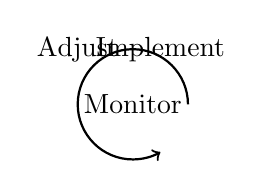
\begin{tikzpicture}[scale=0.7]
                \draw[->,thick] (0,0) arc (0:300:1);
                \node at (-1,0) {Monitor};
                \node at (-2,1) {Adjust};
                \node at (-0.5,1) {Implement};
            \end{tikzpicture}
        \end{column}
    \end{columns}
    
    \begin{exampleblock}{Example}
        Climate change policies adapting to new scientific findings
    \end{exampleblock}
\end{frame}

\begin{frame}{Role-Play: Negotiating a Policy Conflict}
    \begin{block}{Scenario}
        Negotiating climate change policy among stakeholders
    \end{block}
    
    \begin{columns}[T]
        \begin{column}{0.33\textwidth}
            \centering
            \textbf{Industry}\\
            \faIcon[3x]{industry}\\
            Economic Growth
        \end{column}
        \begin{column}{0.33\textwidth}
            \centering
            \textbf{Activist}\\
            \faIcon[3x]{leaf}\\
            Environment
        \end{column}
        \begin{column}{0.33\textwidth}
            \centering
            \textbf{Government}\\
            \faIcon[3x]{balance-scale}\\
            Balance
        \end{column}
    \end{columns}
    
    \begin{alertblock}{Task}
        Develop a policy proposal acceptable to all parties
    \end{alertblock}
\end{frame}

\begin{frame}{Post-Activity Reflection}
    \begin{exampleblock}{Discussion Questions}
        \begin{enumerate}
            \item What strategies worked best in your role?
            \item What challenges did you face in reaching agreement?
            \item How do power imbalances affect real-world negotiations?
        \end{enumerate}
    \end{exampleblock}
    
    \begin{center}
        \faIcon[3x]{comments}
    \end{center}
\end{frame}

\begin{frame}{Discussing Sources of Policy Conflict}
    \begin{columns}[T]
        \begin{column}{0.5\textwidth}
            \textbf{Sources to Consider:}
            \begin{itemize}
                \item Stakeholder interests \faIcon{users}
                \item Ideological differences \faIcon{brain}
                \item Resource limitations \faIcon{coins}
                \item Regulatory constraints \faIcon{gavel}
            \end{itemize}
        \end{column}
        \begin{column}{0.5\textwidth}
            \begin{block}{Discussion Goal}
                Identify patterns and real-world examples to contextualize conflicts
            \end{block}
        \end{column}
    \end{columns}
\end{frame}

\begin{frame}{The Conflict Resolution Pyramid}
    \begin{center}
        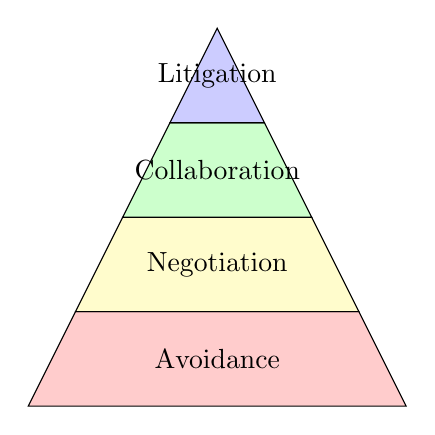
\begin{tikzpicture}[scale=1.2]
            % Draw pyramid levels
            \draw[fill=red!20] (-2,0) -- (2,0) -- (1.5,1) -- (-1.5,1) -- cycle;
            \draw[fill=yellow!20] (-1.5,1) -- (1.5,1) -- (1,2) -- (-1,2) -- cycle;
            \draw[fill=green!20] (-1,2) -- (1,2) -- (0.5,3) -- (-0.5,3) -- cycle;
            \draw[fill=blue!20] (-0.5,3) -- (0.5,3) -- (0,4) -- (-0,4) -- cycle;
            
            % Add labels
            \node at (0,0.5) {Avoidance};
            \node at (0,1.5) {Negotiation};
            \node at (0,2.5) {Collaboration};
            \node at (0,3.5) {Litigation};
        \end{tikzpicture}
    \end{center}
    
    \begin{block}{Key Insight}
        Strategies should match the conflict's scale and importance
    \end{block}
\end{frame}

\begin{frame}{Summary of Key Insights}
    \begin{columns}[T]
        \begin{column}{0.5\textwidth}
            \textbf{Conflict Sources:}
            \begin{itemize}
                \item Stakeholder interests
                \item Ideology
                \item Resources
                \item Regulations
            \end{itemize}
        \end{column}
        \begin{column}{0.5\textwidth}
            \textbf{Management Strategies:}
            \begin{itemize}
                \item Negotiation
                \item Mediation
                \item Collaboration
                \item Litigation
            \end{itemize}
        \end{column}
    \end{columns}
    
    \begin{alertblock}{Opportunities}
        Innovation \faIcon{lightbulb} \quad
        Engagement \faIcon{users} \quad
        Stronger Institutions \faIcon{building}
    \end{alertblock}
\end{frame}

\begin{frame}{Tips for Managing Policy Conflicts}
    \begin{columns}[T]
        \begin{column}{0.5\textwidth}
            \textbf{Skills to Develop:}
            \begin{itemize}
                \item Negotiation \faIcon{handshake}
                \item Communication \faIcon{comments}
            \end{itemize}
        \end{column}
        \begin{column}{0.5\textwidth}
            \textbf{Strategies to Adopt:}
            \begin{itemize}
                \item Flexibility \faIcon{sync}
                \item Evidence-based \faIcon{chart-line}
            \end{itemize}
        \end{column}
    \end{columns}
    
    \begin{exampleblock}{Key Focus}
        Building trust and maintaining open communication
    \end{exampleblock}
\end{frame}

\begin{frame}{Final Reflection}
    \begin{center}
        \textbf{Questions to Consider}
        
        \bigskip
        
        \faIcon[3x]{lightbulb}
    \end{center}
    
    \begin{enumerate}
        \item How can understanding conflict improve your role as a policymaker?
        \item What strategies will you apply in your own policy work?
        \item Can conflict management turn challenges into opportunities?
    \end{enumerate}
    
    \begin{alertblock}{Remember}
        Effective conflict management is key to successful policymaking
    \end{alertblock}
\end{frame}

    \begin{frame}
    \frametitle{Discussion Questions}
    
    \begin{enumerate}
        \item How do you define policy conflict, and what are its key sources?
        \item What are the main strategies for managing policy conflicts, and how do they differ?
        \item Can conflict be both a challenge and an opportunity in the policy-making process? Why or why not?
        \item How can you apply conflict management strategies to a real-world policy issue?
    \end{enumerate}
    \end{frame}

\end{document}